\chapter{Evaluation}
\label{evaluation}

In this chapter, we present and discuss the results of the interview. We evaluate the research questions from the results obtained from the interview. We assess the results by using the correctness of the answers, the time needed and the difficulty rating giving by the interviewees. Correctness is presented in \hyperref[sec:4.1]{Section 4.1} and time measurements is presented in \hyperref[sec:4.2]{Section 4.2}. We also present the results of difficulty rating in \hyperref[sec:4.3]{Section 4.3}. We answer our research question from the presented results in \hyperref[sec:4.4]{Section 4.4}. In \hyperref[sec:4.5]{Section 4.5}, we discuss our findings with respect to the results. We also present certain factors in \hyperref[sec:4.6]{Section 4.6}, that might have influenced our interview unfavorably. Finally, in \hyperref[sec:4.7]{Section 4.7}, we present feedback given by the interviewees on how the visualization of performance-influence model tool can be improved. 

\section{Correctness}
\label{sec:4.1}
We check the answers given by the interviewees to the questions asked in the questionnaire. We evaluate how often an interviewee answered the question correctly. The evaluation is done with respect to each question and each use case; simple and complex. \hyperref[table:correctness]{Table 4.1} presents the relative number of correct answers given for each use case with its summary per question. 
 
\begin{table}[!htbp]
\centering
\small
\begin{tabular}{lccccccc}
\toprule   
 Input & Use Case & Radar Plot  & Text Plot  & Ratio Plot \\ 
\midrule
& Simple & 100\% &  100\% & 88.8\%\\ 
Q1  & Complex &  100\% &  100\% &  77.7\%\\ 
\midrule
& Summary &  100\% &  100\% &  83.83\%\\
\bottomrule
& Simple & 70\% &  100\% & 60\%\\ 
Q2 & Complex & 100\% & 100\% & NA\\ 
\midrule
& Summary & 83.34\% & 100\% &  60\%\\
\bottomrule
& Simple & 100\% &  100\% & 100\%\\ 
Q3 & Complex & 22.23\% & 100\% & 66.66\%\\ 
\midrule
& Summary & 61.11\% & 100\% &  66.66\%\\
\bottomrule
& Simple & 100\% &  88.89\% & 22.23\%\\ 
Q4 & Complex & 88.89\% & 88.89\% & 55.55\%\\ 
\midrule
& Summary & 94.45\% & 88.89\% &  26.66\%\\
\bottomrule
& Simple &  88.89\% &  88.89\% & 33.34\%\\ 
Q5 & Complex & 33.34\% & 100\% &  88.89\%\\ 
\midrule
& Summary & 77.77\% & 94.44\% &  61.11\%\\
\bottomrule
& Simple &  33.34\% &  22.22\% & 88.88\%\\ 
Q6 & Complex & 55.55\% & 77.77\% &  77.77\%\\ 
\midrule
& Summary & 61.11\% & 50\% & 83.33\%\\
\bottomrule
\end{tabular}
\label{table:correctness}
\caption[Correctness Table]{The relative number of correctly answered questions in the interview for the different visualization techniques
across the different questions and complexities.} 
\end{table}
 
\section{Time Measurements}
\label{sec:4.2}
The second factor to evaluate the research questions, is by taking time measurements.

\begin{table}[!htbp]
\centering
\begin{adjustbox}{width=1\textwidth}
\begin{tabular}{@{\extracolsep{4pt}}lccccccc}
\toprule   
   &  Radar Plot  & Text Plot  & Ratio Plot  & Radar Plot  & Text Plot  & Ratio Plot \\ 
Input & <  & <  & < & > & > & > \\
   &  Text Plot & Ratio Plot & Radar Plot & Text Plot & Ratio Plot & Radar Plot\\
\midrule
Q1 Simple  & 0.535 & 0.638 & 0.5 & 0.5 & 0.395 & 0.535\\ 
Q1 Complex & 0.535 & 0.464 & 0.604 & 0.5 & 0.570 & 0.429\\ 
Q2 Simple  &  0.855 & \textbf{0.010} & 0.953 & 0.165 & 0.991 & \textbf{0.055}\\ 
Q2 Complex & 0.811 & \textbf{--} & \textbf{--} & 0.213 & \textbf{--} & \textbf{--}\\ 
Q3 Simple  & 0.5 & \textbf{0.004} & 0.994 & 0.535 & 0.996 & \textbf{0.006}\\ 
Q3 Complex & 0.982  & \textbf{0.004} & 0.701 & \textbf{0.021} & 0.996 & 0.329\\ 
Q4 Simple & 0.395 & \textbf{0.001} &  0.999 & 0.638 & 0.998 & \textbf{0.000}\\ 
Q4 Complex & 0.638 & \textbf{0.006} & 0.996 & 0.395 & 0.994 &  \textbf{0.004}\\ 
Q5 Simple  & 0.973 & 0.055 & 0.701 & \textbf{0.031} & 0.953 & 0.329\\ 
Q5 Complex & 0.429 & 0.125 & 0.670 & 0.604 & 0.891 & 0.361\\ 
Q6 Simple  & 0.464 & 0.760 & 0.329 & 0.570 & 0.268 & 0.701\\ 
Q6 Complex & 0.535 & 0.188 &  0.811 & 0.5 & 0.834 & 0.213 \\ 
 \midrule
Q1 Simple \& Complex & 0.581 & 0.493 &  0.544 & 0.430 & 0.581 & 0.468\\ 
Q2 Simple \& Complex & 0.920 & \textbf{0.004} &  0.973 & 0.084 & 0.995 &  \textbf{0.030}\\ 
Q3 Simple \& Complex & 0.894 & \textbf{0.000} & 0.976 & 0.111 & 0.999 & \textbf{0.025}\\
Q4 Simple \& Complex & 0.518 & \textbf{0.000} &  0.999 & 0.493 & 0.999 & \textbf{0.000} \\
Q5 Simple \& Complex & 0.899 & \textbf{0.028} & 0.559 & 0.105 & 0.973 &  0.454\\
Q6 Simple \& Complex & 0.455 & 0.369 & 0.665 & 0.556 & 0.642 & 0.346\\
\bottomrule
\end{tabular}
\end{adjustbox}
\label{table:time}
\caption[Mann-Whitney U Test]{Mann-Whitney U test results for the different visualization techniques across the different questions and complexities.} 
\end{table}

Time is measured on how long an interviewee took to answer a question. This is done to compare if an interviewee took a long time to answer a complex use case than a simpler one or to check if one of the visualization techniques was more time consuming than others.

We will conduct the \textit{Mann–Whitney U test} in this section.

\subsection{Mann–Whitney U test}
We use the Mann-Whitney U test to determine if one sample is significantly better than another sample when time is considered as a factor. A sample is significantly better than another if the p value of the test is less than 0.05. \hyperref[table:time]{Table 4.2}, presents the results for Mann–Whitney U test. The significant values are marked in bold.

In our case, we determine if one group of time measurement is significantly better than another group of time measurement. We compare time measurement groups between the radar plot, the text plot, and the ratio plot. 

Here we try to find, if a visualization technique consumed significantly less time than other visualization techniques. For instance, radar plot $<$ text plot implies if the radar plot is better than the text plot if the Mann–Whitney U test value is less 0.05. Similarly, radar plot $>$ text plot implies if the radar plot is worse than the text plot. 

\section{Difficulty Rating}
\label{sec:4.3}

The difficulty rating in our thesis is assessed using Likert scales. This scale helps us determine the difficulty perception of the interviewee based on the visualization technique and the complexity of the performance-influence model.

The difficulty rating is considered as a factor for the evaluation of research questions. The interviewee selects the difficulty rating on how easy or difficult it was to answer a question. This rating corresponds to the time taken by the interviewee to answer the question. \hyperref[table:rating]{Table 4.3}, we present the average difficulty ratings and their standard deviation.

\begin{table}[!htbp]
\centering
\small
\begin{tabular}{@{\extracolsep{4pt}}lccccccc}
\toprule   
{} & \textbf{Radar Plot} &   &   \textbf{Text Plot} &   &  \textbf{Ratio Plot}\\
 \cmidrule{2-3} 
 \cmidrule{4-5} 
  \cmidrule{6-7} 
Input  &  Mean $\varpm$ SD & & Mean $\varpm$ SD & & Mean $\varpm$ SD \\
\midrule
Q1 Simple  & $1.3\varpm 0.471$ &  & $1.5\varpm 0.496$ &  &   $1.2\varpm 0.415$& \\ 
Q1 Complex & $2.4\varpm 0.831$ &  & $2.2\varpm 0.628$ &  &   $1.3\varpm 0.471$& \\ 
Q2 Simple  & $1.5\varpm 0.684$ &  & $1.5\varpm 0.831$ &  &   $4.2\varpm 1.030$& \\ 
Q2 Complex & $1.8\varpm 0.566$ &  & $2.0\varpm 0.471$ &  & \textbf{--} & \\ 
Q3 Simple  & $1.5\varpm 0.496$ &  & $1.6\varpm 0.666$ &  &   $3.1\varpm 1.286$& \\ 
Q3 Complex & $2.8\varpm 1.099$ &  & $2.1\varpm 0.314$ &  &   $3.4\varpm 1.065$& \\ 
Q4 Simple  & $1.6\varpm 0.471$ &  & $1.7\varpm 0.415$ &  &   $3.7\varpm 0.916$& \\ 
Q4 Complex & $2.4\varpm 0.496$ &  & $1.8\varpm 0.314$ &  &   $3.5\varpm 0.955$& \\  
Q5 Simple  & $2.6\varpm 1.054$ &  & $2.2\varpm 0.785$ &  &   $4.3\varpm 0.942$& \\  
Q5 Complex & $2.8\varpm 0.993$ &  & $1.7\varpm 0.628$ &  &   $4.4\varpm 0.684$& \\ 
Q6 Simple  & $2.7\varpm 0.628$ &  & $3.0\varpm 0.666$ &  &   $3.6\varpm 1.054$& \\ 
Q6 Complex & $2.3\varpm 0.471$ &  & $2.5\varpm 0.955$ &  &   $4.2\varpm 1.030$& \\ 
 \midrule
Q1 Simple \& Complex  & $1.8\varpm 0.874$ &  & $1.8\varpm 0.657$ &  &   $1.2\varpm 0.447$& \\ 
Q2 Simple \& Complex  & $1.7\varpm 0.650$ &  & $1.7\varpm 0.711$ &  &   $4.2\varpm 1.030$& \\ 
Q3 Simple \& Complex  & $2.2\varpm 1.082$ &  & $1.8\varpm 0.566$ &  &   $3.2\varpm 1.192$& \\ 
Q4 Simple \& Complex  & $2.0\varpm 0.621$ &  & $1.8\varpm 0.372$ &  &   $3.6\varpm 0.942$& \\
Q5 Simple \& Complex  & $2.7\varpm 1.030$ &  & $2.0\varpm 0.745$ &  &   $4.3\varpm 0.825$& \\
Q6 Simple \& Complex  & $2.5\varpm 0.598$ &  & $2.7\varpm 0.853$ &  &   $3.9\varpm 1.078$& \\ 
\bottomrule
\end{tabular}
\label{table:rating}
\caption[Average difficulty Rating]{Average difficulty rating and their standard deviations for all interviewees. The mean and standard deviations are computed for each different visualization techniques across the different questions and complexities.} 
\end{table}

\subsection{Pearson Correlation Coefficient}
We compute the Pearson correlation coefficient~\cite{pearson1896vii} with difficulty ratings and time measurements as input. This coefficient is used to determine the measure of linear correlation between the 2 inputs. \hyperref[table:pearons]{Table 4.4}, presents the linear correlation values for the same.

The coefficient ranges from -1 to +1. A value of less than 0.5 implies a weak correlation, a value between 0.5 - 0.8 implies medium correlation and value greater than 0.8 implies a strong correlation. A positive coefficient implies that both inputs increase or decrease linearly and a negative coefficient implies that both increase or decrease inversely.

From \hyperref[table:pearons]{Table 4.4}, we can see that the only strong correlation coefficient is between the time measurements and difficulty ratings of Q3 for a simple use case with the radar plot as the visualization technique.

\begin{table}[!htbp]
\centering
\begin{tabular}{@{\extracolsep{4pt}}lccccccc}
\toprule   
{} & \textbf{Radar Plot} &   &   \textbf{Text Plot} &   &  \textbf{Ratio Plot}\\
 \cmidrule{2-3} 
 \cmidrule{4-5} 
  \cmidrule{6-7} 
Input  & Coefficient &  & Coefficient &  & Coefficient \\
\midrule
Q1 Simple  & -0.013 &  & 0.216 &  & 0.711 & \\ 
Q1 Complex & 0.637 &  & 0.403 &  & -0.218 & \\ 
Q2 Simple  & 0.384 &  & -0.280 &  & -0.019 & \\ 
Q2 Complex & 0.753 &  & 0.576 &  & \textbf{--} & \\ 
Q3 Simple  & 0.877 &  & 0.566 &  & 0.506 & \\ 
Q3 Complex & 0.163 &  & 0.509 &  & 0.119 & \\ 
Q4 Simple  & 0.350 &  & 0.347 &  & 0.626 &\\ 
Q4 Complex & -0.268 &  & 0.373 &  & -0.280 &\\ 
Q5 Simple  & 0.289 &  & 0.493 &  & 0.401 &\\ 
Q5 Complex & 0.618 &  & 0.773 &  & -0.133 &\\ 
Q6 Simple  & -0.145 &  & -0.268  &  & 0.519 &\\ 
Q6 Complex & 0.293 &  & 0.178  &  & 0.487 &\\ 
\bottomrule
\end{tabular}
\label{table:pearons}
\caption[Pearson correlation coefficient]{Pearson correlation coefficient for the different visualization techniques across the different questions and complexities.} 
\end{table}

Time measurements and difficulty ratings are also plotted for each interviewee, for each question. This is done so as to look at the correlation between them graphically. These plots are presented in \hyperref[sanityCheck]{Appendix:A.2}

\section{Results}
\label{sec:4.4}

We now answer the research questions by using the results from the correctness values, the time measurements, and the difficulty ratings.

We also use Pareto front plots for each research question. So far we have considered the two evaluation factors; correctness and time separately. Using Pareto front plots, we combine these two factors. These plots are plotted with time vs correctness. They help us to determine which visualization technique is the best when considering both these evaluation factors. Visualization is considered the best when it takes the lowest amount of time to answer a question with the the highest relative number of correct values.

\subsection*{One Performance-Influence Model}
\vskip 0.2in
\begin{mdframed}
\textbf{RQ1: Can we use the visualization techniques to identify relevant configuration options or interactions  of one performance-influence model?}
\end{mdframed}

We consider Q1 and Q2 for this research question.

\vskip 0.2in
\begin{mdframed}
\textbf{RQ1.1: Can we use the visualization techniques to identify relevant configuration options or interactions  of one simple performance-influence model?}
\end{mdframed}

For this sub-question, we only consider the simple use case for Q1 and Q2.

\begin{description}[leftmargin=0pt]
\item[Correctness: ]From \hyperref[table:correctness]{Table 4.1}, we can infer that all the interviewees were able to answer Q1 and Q2 correctly when presented with the text plot as the visualization technique. Whereas, the ratio plot did not perform as good as the text plot for both Q1 and Q2.

\item[Time Measurements: ]From the results presented in \hyperref[table:time]{Table 4.2}, we can see that only for Q2, the text plot proved to be significantly better than other visualization techniques.

\item[Difficulty Ratings: ]From the difficulty ratings presented in \hyperref[table:rating]{Table 4.3}, we can note that the average difficulty ratings for Q1 and Q2 are below 2.4 with an exception of the ratio plot for Q2. Where it has an average rating of 4.2, but also with a higher standard deviation.

\end{description}

\textbf{Q1}: From \hyperref[figure:paretoOneQ1]{Figure 4.1}, for the simple use case the text plot is much better than other visualization techniques. We can also notice that the ratio plot takes slightly less time, but does not guarantee perfect correctness results.

\textbf{Q2}: From \hyperref[figure:paretoOneQ2]{Figure 4.2}, for the simple use case, the text plot is much better both in terms of time and correctness. 

\textbf{Summary of RQ1.1}: The answer to this sub-question is \textbf{yes}, with the text plot being the choice of visualization.

\begin{figure}[hbt!]
\centering
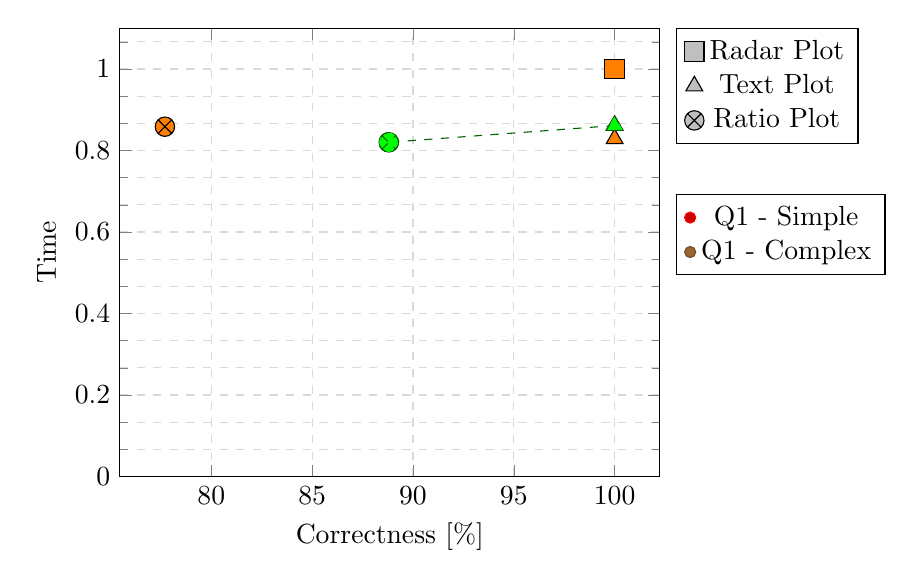
\begin{tikzpicture}
\definecolor{clr1}{RGB}{0,100,0}
\definecolor{clr2}{RGB}{255,165,0}
	\begin{axis}[%
	xlabel={Correctness [\%]},
    ylabel={Time},
    ymin=0,
    minor y tick num=2,
    grid style={dashed,gray!30},
    ymajorgrids=true,
    xmajorgrids=true,
    yminorgrids=true,
    only marks,
    scatter,
    mark size=3.5pt,
    scatter src=explicit symbolic,
	scatter/classes={
		x={mark=square*,fill=lightgray},
		y={mark=triangle*,fill=lightgray},
		z={mark=otimes*,fill=lightgray},
		a={mark=square*,fill=green},
		b={mark=triangle*,fill=green},
		c={mark=otimes*,fill=green},
		d={mark=square*,fill=orange},
		e={mark=triangle*,fill=orange},
		f={mark=otimes*,fill=orange}},
	     legend entries={
            Radar Plot,
            Text Plot,
            Ratio Plot%
        },
        legend pos=outer north east,]
	\addplot[scatter,only marks,%
		scatter src=explicit symbolic]%
	table[meta=label] {
x         y         label
100       1         a  
100       0.8612    b 
88.8      0.8201    c 
100       1         d 
100       0.8288    e 
77.7      0.8584    f 
};
\addplot +[clr1, smooth, dashed] table[meta=label]  {
x          y         label 
100       0.8612      b 
88.8      0.8201      c 
}; 
\end{axis}
	
\begin{axis}[
    xmin=0,
    xmax=100,
    ymin=1,
    ymax=6,
    hide axis,
    only marks,
    legend entries={
     ,       % the dummy plot should not show up in the legend
        Q1 - Simple,
        Q1 - Complex,%  
    },
     legend pos=outer north east,
    legend style={
            yshift=-60pt,
        },
    ]
\foreach \i in {0,...,6} {
        \addplot+ [mark=*] coordinates { (0,0) };
     }
    \end{axis}
\end{tikzpicture}
\label{figure:paretoOneQ1}
\caption[Pareto front for Q1]{The correctness and time values for Q1 (simple and complex). The Pareto front for the different complexities is drawn by using a green and orange line respectively. The visualizations on the Pareto front for Q1 - Simple is text and the ratio plot and for Q1 - Complex is the text plot.} 
\end{figure}

\begin{figure}[hbt!]
\centering
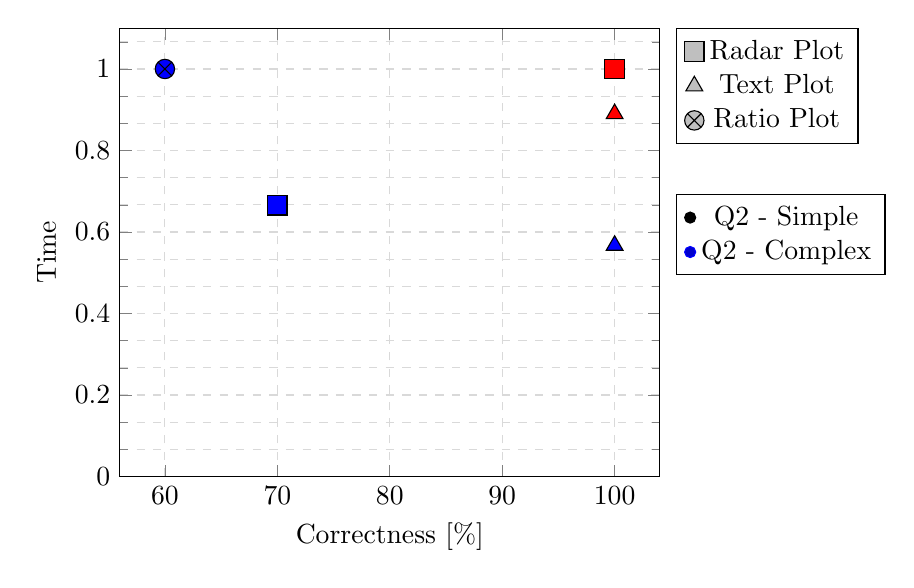
\begin{tikzpicture}
	\begin{axis}[%
	xlabel={Correctness [\%]},
    ylabel={Time},
    ymin=0,
    minor y tick num=2,
    grid style={dashed,gray!30},
    ymajorgrids=true,
    xmajorgrids=true,
    yminorgrids=true,
    only marks,
    scatter,
    mark size=3.5pt,
    scatter src=explicit symbolic,
	scatter/classes={
		x={mark=square*,fill=lightgray},
		y={mark=triangle*,fill=lightgray},
		z={mark=otimes*,fill=lightgray},
		g={mark=square*,fill=blue},
	    h={mark=triangle*,fill=blue},
		i={mark=otimes*,fill=blue},
		j={mark=square*,fill=red},
	    k={mark=triangle*,fill=red}},
	     legend entries={
            Radar Plot,
            Text Plot,
            Ratio Plot%
        },
        legend pos=outer north east,]
	\addplot[scatter,only marks,%
		scatter src=explicit symbolic]%
	table[meta=label] {
x         y         label
70        0.6656    g  
100       0.567     h 
60        1         i 
100       1         j 
100       0.89      k 
};
\end{axis}
	
\begin{axis}[
    xmin=0,
    xmax=100,
    ymin=1,
    ymax=6,
    hide axis,
    only marks,
    legend entries={
     ,   ,  ,  % the dummy plot should not show up in the legend
        Q2 - Simple,
        Q2 - Complex%
    },
     legend pos=outer north east,
    legend style={
            yshift=-60pt,
        },
    ]
\foreach \i in {0,...,6} {
        \addplot+ [mark=*] coordinates { (0,0) };
     }
    \end{axis}
\end{tikzpicture}
\label{figure:paretoOneQ2}
\caption[Pareto front for Q2]{The correctness and time values for Q2 (simple and complex). The Pareto front for the different complexities is drawn by using a blue and red line respectively. The visualizations on the Pareto front for Q2 - Simple is the text plot and for Q2 - Complex is the text plot.} 
\end{figure}

\vskip 0.2in
\begin{mdframed}
\textbf{RQ1.2: Can we use the visualization techniques to identify relevant configuration options or interactions  of one complex performance-influence model?}
\end{mdframed}

For this sub-question, we only consider the complex use case for Q1 and Q2.

\begin{description}[leftmargin=0pt]
\item[Correctness: ] From \hyperref[table:correctness]{Table 4.1}, we can infer that all the interviewees were able to answer the Q1 and Q2 correctly for both the radar plot and the text plot. 

\item[Time Measurements: ] From the results presented in \hyperref[table:time]{Table 4.2}, we can see infer that none of the visualization technique proved to be significantly better than the other visualization techniques. 

\item[Difficulty Ratings: ] From the difficulty ratings presented in \hyperref[table:rating]{Table 4.3}, we can infer that all of the 3 visualization techniques had an average difficulty rating below 2.4
\end{description}

\textbf{Q1}: From \hyperref[figure:paretoOneQ1]{Figure 4.1}, we can notice that for the complex use case, both the radar plot and the text plot perform equally better in terms of correctness. However, the text plot performed slightly better in terms of time. Whereas, the ratio plot did not perform as good as text and the radar plot.

\textbf{Q2}: From \hyperref[figure:paretoOneQ2]{Figure 4.2}, for the complex use case, the text plot is slightly better than the radar plot both in terms of time and correctness. The ratio plot was not considered for this question, since the ratio plot displays the general influence of a configuration option or interaction, also that the ratio plot does not display configuration options with zero or no influence.

\textbf{Summary of RQ1.2}: The answer to this sub-question is \textbf{yes}, with the text plot being the choice of visualization.

\textbf{Summary of RQ1}: Hence, the answer to this research question is \textbf{yes}, with the text plot being the considerable choice of visualization, since it has better results when considering time, correctness, and difficulty rating factors.

\subsection*{Two Performance-Influence Models}
\vskip 0.2in
\begin{mdframed}
\textbf{RQ2: Can we use the visualization to compare two performance-influence models?}
\end{mdframed}

We consider Q3 and Q4 for this research question.

\vskip 0.2in
\begin{mdframed}
\textbf{RQ2.1: Can we use the visualization to compare two simple performance-influence models?}
\end{mdframed}

For this sub-question, we consider only the simple use case for Q3 and Q4.

\begin{description}[leftmargin=0pt]
\item[Correctness: ] From \hyperref[table:correctness]{Table 4.1}, we can infer that for Q3 all the interviewees answered correctly when presented with any of the 3 visualization techniques, whereas for Q4 only the radar plot performed better than the text plot and the ratio plot.

\item[Time Measurements: ] From the results presented in \hyperref[table:time]{Table 4.2}, we can see that the text plot performed significantly better in terms of time measurements.

\item[Difficulty Ratings: ] From the difficulty ratings presented in \hyperref[table:rating]{Table 4.3}, we can see that the ratio plot has on an average higher difficulty rating than the text plot and the radar plot.

\end{description}


\textbf{Q3:} From \hyperref[figure:paretoTwoQ3]{Figure 4.3}, for the simple use case, we can infer that both the text plot and the radar plot are equally better when both factors; correctness and time are considered. We also see that both these visualization techniques produce perfect correctness results.

\textbf{Q4:} From \hyperref[figure:paretoTwoQ4]{Figure 4.4}, for the simple use case, the radar plot is better in terms of correctness measurements. But, from \hyperref[table:time]{Table 4.2}, we know the text plot does significantly better than other visualization techniques. This implies that even though interviewees took less time to answer the text plot, the results were not 100\% correct.

\textbf{Summary of RQ2.1}: Therefore, the answer to this sub-question is \textbf{yes}, with the text plot being the considerable choice of visualization.

\begin{figure}[hbt!]
\centering
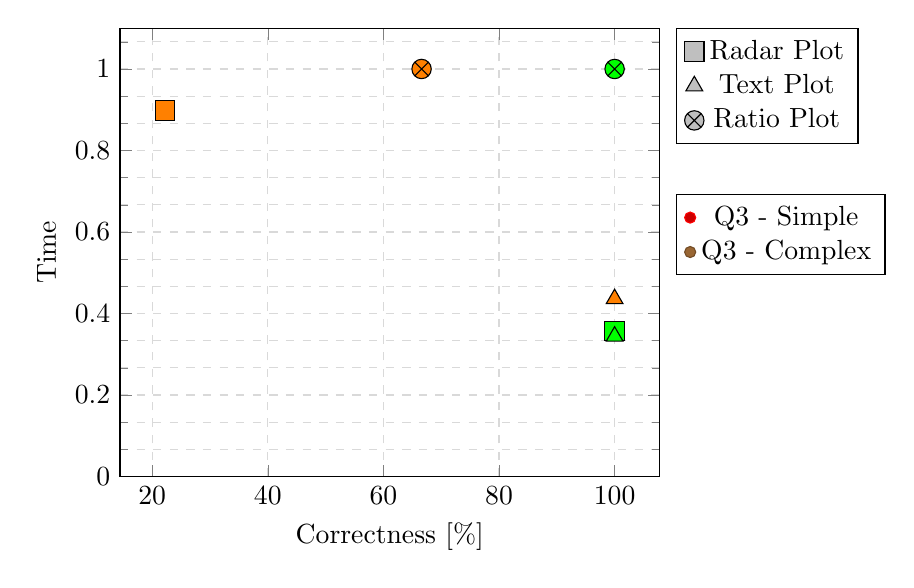
\begin{tikzpicture}
	\begin{axis}[%
	xlabel={Correctness [\%]},
    ylabel={Time},
    ymin=0,
    minor y tick num=2,
    grid style={dashed,gray!30},
    ymajorgrids=true,
    xmajorgrids=true,
    yminorgrids=true,
    only marks,
    scatter,
    mark size=3.5pt,
    scatter src=explicit symbolic,
	scatter/classes={%
		x={mark=square*,fill=lightgray},
		y={mark=triangle*,fill=lightgray},
		z={mark=otimes*,fill=lightgray},
		a={mark=square*,fill=green},%
		b={mark=triangle*,fill=green},%
		c={mark=otimes*,fill=green},%
		d={mark=square*,fill=orange},%
		e={mark=triangle*,fill=orange},%
		f={mark=otimes*,fill=orange}},
	     legend entries={
            Radar Plot,
            Text Plot,
            Ratio Plot%
        },
        legend pos=outer north east,]]
	\addplot[scatter,only marks,%
		scatter src=explicit symbolic]%
	table[meta=label] {
x         y            label
100       0.357        a  
100       0.344        b 
100       1            c 
22.20     0.898        d 
100       0.436        e 
66.6      1            f 
	};
	
\end{axis}

\begin{axis}[
    xmin=0,
    xmax=100,
    ymin=1,
    ymax=6,
    hide axis,
    only marks,
    legend entries={
     ,       % the dummy plot should not show up in the legend
        Q3 - Simple,
        Q3 - Complex,%
    },
     legend pos=outer north east,
    legend style={
            yshift=-60pt,
        },
    ]
\foreach \i in {0,...,6} {
        \addplot+ [mark=*] coordinates { (0,0) };
     }
    \end{axis}
\end{tikzpicture}
\label{figure:paretoTwoQ3}
\caption[Pareto front for Q3]{The correctness and time values for Q3 (simple and complex). The Pareto front for the different complexities is drawn  by using a green and orange line respectively. The visualizations on the Pareto front for Q3 - Simple is the radar and the text plot and for Q3 - Complex is the text plot.} 
\end{figure}

\begin{figure}[hbt!]
\centering
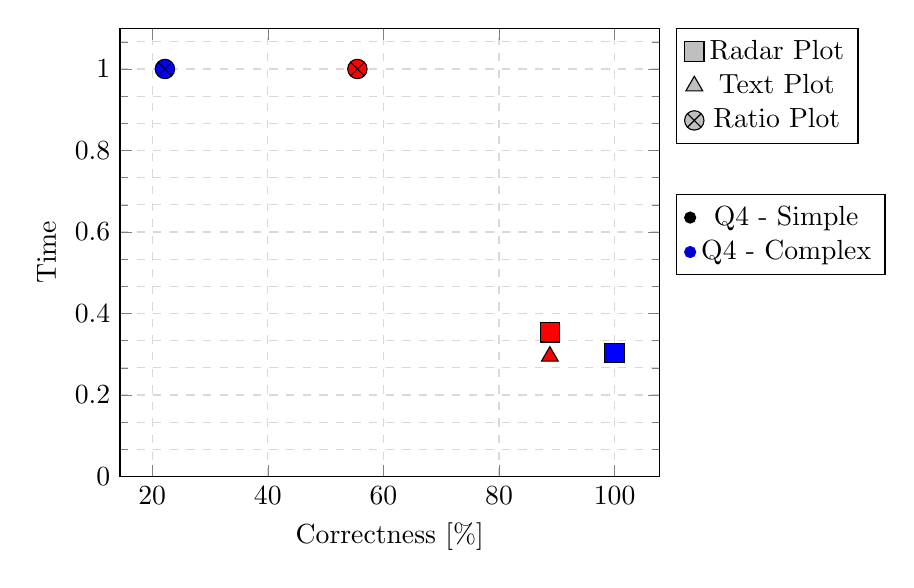
\begin{tikzpicture}
	\begin{axis}[%
	xlabel={Correctness [\%]},
    ylabel={Time},
    ymin=0,
    minor y tick num=2,
    grid style={dashed,gray!30},
    ymajorgrids=true,
    xmajorgrids=true,
    yminorgrids=true,
    only marks,
    scatter,
    mark size=3.5pt,
    scatter src=explicit symbolic,
	scatter/classes={%
		x={mark=square*,fill=lightgray},
		y={mark=triangle*,fill=lightgray},
		z={mark=otimes*,fill=lightgray},
		g={mark=square*,fill=blue},%
	    h={mark=triangle*,fill=blue},%
		i={mark=otimes*,fill=blue},%
		j={mark=square*,fill=red},%
	    k={mark=triangle*,fill=red},%
	    l={mark=otimes*,fill=red}},
	     legend entries={
            Radar Plot,
            Text Plot,
            Ratio Plot%
        },
        legend pos=outer north east,]]
	\addplot[scatter,only marks,%
		scatter src=explicit symbolic]%
	table[meta=label] {
x         y            label
100       0.303        g  
88.80     0.354        h 
22.20     1            i 
88.80     0.354        j 
88.80     0.295        k 
55.50     1            l 
	};

\end{axis}

\begin{axis}[
    xmin=0,
    xmax=100,
    ymin=1,
    ymax=6,
    hide axis,
    only marks,
    legend entries={
     ,   , ,    % the dummy plot should not show up in the legend
        Q4 - Simple,
        Q4 - Complex%
    },
     legend pos=outer north east,
    legend style={
            yshift=-60pt,
        },
    ]
\foreach \i in {0,...,6} {
        \addplot+ [mark=*] coordinates { (0,0) };
     }
    \end{axis}
\end{tikzpicture}
\label{figure:paretoTwoQ4}
\caption[Pareto front for Q4]{The correctness and time values for Q4 (simple and complex). The Pareto front for the different complexities is drawn by using a blue and red line respectively. The visualizations on the Pareto front for Q4 - Simple is the radar plot and for Q4 - Complex is the text plot.}
\end{figure}

\vskip 0.2in
\begin{mdframed}
\textbf{RQ2.2: Can we use the visualization to compare two complex performance-influence models?}
\end{mdframed}

For this sub-question, we consider only the complex use case for Q3 and Q4.

\begin{description}[leftmargin=0pt]
\item[Correctness: ] From \hyperref[table:correctness]{Table 4.1}, we can infer that for Q3, all the interviewees answered correctly when presented with the text plot. Whereas, for Q4 none of the visualization techniques gave perfect correctness answers.

\item[Time Measurements: ] From the results presented in \hyperref[table:time]{Table 4.2}, we can see that the text plot performed significantly better in terms of time measurements.

\item[Difficulty Ratings: ] From the difficulty ratings presented in \hyperref[table:rating]{Table 4.3}, we can see that the ratio plot has on an average higher difficulty rating than the text plot and the radar plot.

\end{description}

\textbf{Q3:} From \hyperref[figure:paretoTwoQ3]{Figure 4.3}, for the complex use case, we can infer that both the text plot outperformed other visualization techniques when both factors; correctness and time are considered.

\textbf{Q4:} From \hyperref[figure:paretoTwoQ4]{Figure 4.4}, for the complex use case, we can infer that the text plot is slightly better than the radar plot both in terms of time and correctness factors, even though it did not lead to perfect correctness results.

\textbf{Summary of RQ2.2}: Therefore, the answer to this sub-question is \textbf{yes}.

\textbf{Summary of RQ2}: Hence, the answer to this research question is \textbf{yes}, with the text plot being the considerable choice of visualization technique, since it has better results when considering time, correctness, and difficulty ratings.

\subsection*{Many Performance-Influence Models}

\vskip 0.2in
\begin{mdframed}
\textbf{RQ3: How good can the visualizations be used to compare a high number of performance-influence models and a high number of terms?}
\end{mdframed}

We consider Q5 and Q6 for this research question.

Q5 corresponds to scalability with respect to the addition of performance-influence models and Q6 corresponds to scalability with respect to the addition of configuration option or interactions.

\begin{mdframed} 
\textbf{RQ3.1: How good can the visualizations be used to compare a high number of simple performance-influence models and a high number of terms?}
\end{mdframed}

For this sub-question, we only consider the simple use case for Q5 and Q6.

\begin{description}[leftmargin=0pt]
\item[Correctness: ] From \hyperref[table:correctness]{Table 4.1}, we can infer that for both Q5 and Q6, none of the visualization techniques lead to perfect correctness answer. Although, the text plot performed comparatively better for Q5 and the ratio plot performed comparatively better for Q6.

\item[Time Measurements: ] From the results presented in \hyperref[table:time]{Table 4.2}, none of the visualization techniques performed significantly better in terms of time measurements.

\item[Difficulty Ratings: ] From the difficulty ratings presented in \hyperref[table:rating]{Table 4.3}, we can infer that the ratio plot has higher difficulty ratings for Q5 and Q6.

\end{description}

\textbf{Q5:} From \hyperref[figure:paretoManyQ5]{Figure 4.5}, for the simple use case, we can see that the text plot is a better choice of visualization technique when considering both time and correctness factors.

\textbf{Q6:} From \hyperref[figure:paretoManyQ6]{Figure 4.6}, for the simple use case, we can infer that if time is considered as a factor, the radar plot performs comparatively better than other visualization techniques. However, when correctness is considered as a factor, the ratio plot performs better. Even though both these plots do not lead to perfect correctness results.

\textbf{Summary of RQ3.1}: The answer to this sub-question is \textbf{yes}, with the text plot as the best visualization type for performance-influence models with many terms and the ratio plot as the best visualization for many performance-influence models.


\begin{figure}[hbt!]
\centering
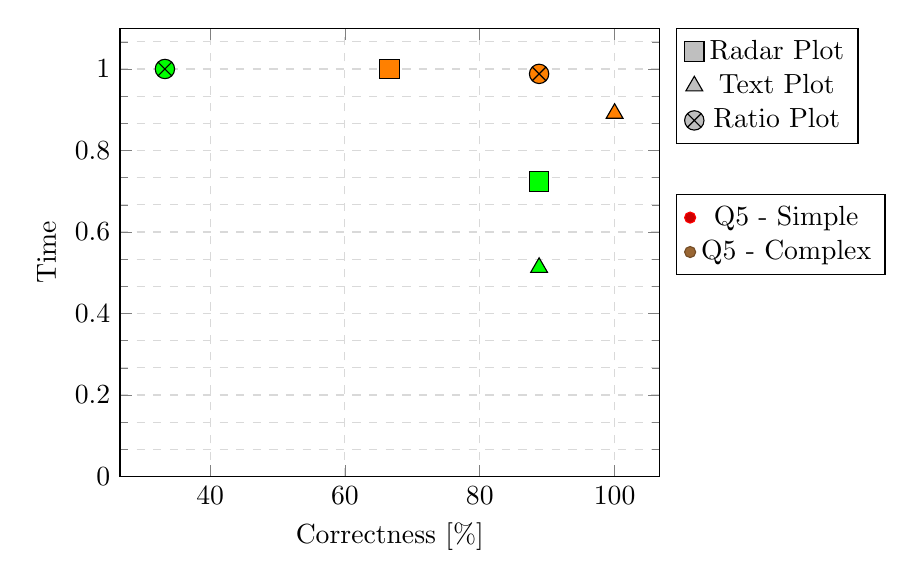
\begin{tikzpicture}
	\begin{axis}[%
	xlabel={Correctness [\%]},
    ylabel={Time},
    ymin=0,
    minor y tick num=2,
    grid style={dashed,gray!30},
    ymajorgrids=true,
    xmajorgrids=true,
    yminorgrids=true,
    only marks,
    scatter,
    mark size=3.5pt,
    scatter src=explicit symbolic,
	scatter/classes={%
		x={mark=square*,fill=lightgray},
		y={mark=triangle*,fill=lightgray},
		z={mark=otimes*,fill=lightgray},
		a={mark=square*,fill=green},%
		b={mark=triangle*,fill=green},%
		c={mark=otimes*,fill=green},%
		d={mark=square*,fill=orange},%
		e={mark=triangle*,fill=orange},%
		f={mark=otimes*,fill=orange}},
	     legend entries={
            Radar Plot,
            Text Plot,
            Ratio Plot%
        },
        legend pos=outer north east,]]
	\addplot[scatter,only marks,%
		scatter src=explicit symbolic]%
	table[meta=label] {
x         y            label
88.80     0.724        a  
88.80     0.513        b 
33.30     1            c 
66.60     1            d 
100       0.891        e 
88.80     0.988        f 
	};
	\end{axis}
\begin{axis}[
    xmin=1,
    xmax=100,
    ymin=1,
    ymax=6,
    hide axis,
    only marks,
    legend entries={
     ,       % the dummy plot should not show up in the legend
        Q5 - Simple,
        Q5 - Complex%
    },
     legend pos=outer north east,
    legend style={
            yshift=-60pt,
        },
    ]
\foreach \i in {0,...,6} {
        \addplot+ [mark=*] coordinates { (0,0) };
     }
    \end{axis}
\end{tikzpicture}
\label{figure:paretoManyQ5}
\caption[Pareto front for Q5]{The correctness and time values for Q5 (simple and complex). The pareto front for the different complexities is drawn by using a green and orange line respectively. The visualizations on the pareto front for Q5 - Simple is the text plot and for Q5 - Complex is the text plot.} 
\end{figure}

\begin{figure}[hbt!]
\centering
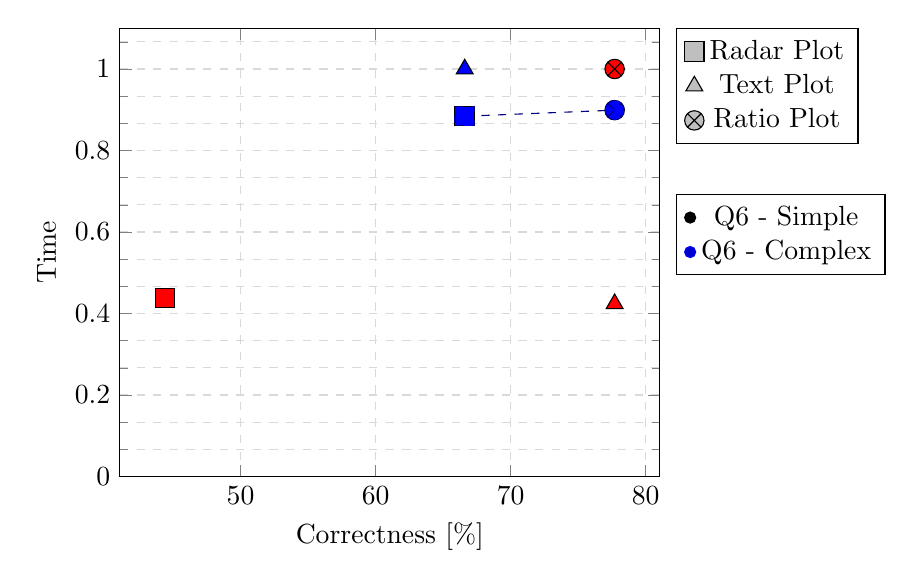
\begin{tikzpicture}
\definecolor{clr1}{RGB}{139,0,0}    
\definecolor{clr2}{RGB}{0,0,128} 
	\begin{axis}[%
	xlabel={Correctness [\%]},
    ylabel={Time},
    ymin=0,
    minor y tick num=2,
    grid style={dashed,gray!30},
    ymajorgrids=true,
    xmajorgrids=true,
    yminorgrids=true,
    only marks,
    scatter,
    mark size=3.5pt,
    scatter src=explicit symbolic,
	scatter/classes={%
		x={mark=square*,fill=lightgray},
		y={mark=triangle*,fill=lightgray},
		z={mark=otimes*,fill=lightgray},
		g={mark=square*,fill=blue},%
	    h={mark=triangle*,fill=blue},%
		i={mark=otimes*,fill=blue},%
		j={mark=square*,fill=red},%
	    k={mark=triangle*,fill=red},%
	    l={mark=otimes*,fill=red}},
	     legend entries={
            Radar Plot,
            Text Plot,
            Ratio Plot%
        },
        legend pos=outer north east,]]
	\addplot[scatter,only marks,%
		scatter src=explicit symbolic]%
	table[meta=label] {
x         y            label
66.60     0.884        g  
66.60     1            h 
77.70     0.899        i 
44.40     0.438        j 
77.70     0.424        k 
77.70     1            l 
	};
\addplot +[clr2, smooth, dashed] table[meta=label]  {
x          y         label 
66.60     0.884        g  
77.70     0.899        i 
}; 	
	\end{axis}
\begin{axis}[
    xmin=0,
    xmax=100,
    ymin=1,
    ymax=6,
    hide axis,
    only marks,
    legend entries={
     ,  ,  ,     % the dummy plot should not show up in the legend
        Q6 - Simple,
        Q6 - Complex%
    },
     legend pos=outer north east,
    legend style={
            yshift=-60pt,
        },
    ]
\foreach \i in {0,...,6} {
        \addplot+ [mark=*] coordinates { (0,0) };
     }
    \end{axis}
\end{tikzpicture}
\label{figure:paretoManyQ6}
\caption[Pareto front for Q6]{The correctness and time values for Q6 (simple and complex). The Pareto front for the different complexities is drawn by  using a blue and red line respectively. The visualizations on the Pareto front for Q6 - Simple is the radar and the ratio plot and for Q6 - Complex is the text plot.} 
\end{figure}
 
\begin{mdframed} 
\textbf{RQ3.2: How good can the visualizations be used to compare a high number of complex performance-influence models and a high number of terms?}
\end{mdframed}

For this sub-question, we only consider the complex use case for Q5 and Q6.

\begin{description}[leftmargin=0pt]
\item[Correctness: ] From \hyperref[table:correctness]{Table 4.1}, we can infer that for Q5, all the interviewees were able to answer the question correctly when presented with the text plot. However, for Q6, the ratio plot and the text plot performed equally good, even though both did not lead to perfect correctness results.

\item[Time Measurements: ] From the results presented in \hyperref[table:time]{Table 4.2}, none of the visualization techniques performed significantly better in terms of time measurements.

\item[Difficulty Ratings: ] From the difficulty ratings presented in \hyperref[table:rating]{Table 4.3}, we can infer that the ratio plot has higher difficulty ratings for Q5 and Q6.

\end{description}

\textbf{Q5:} From \hyperref[figure:paretoManyQ5]{Figure 4.5}, for the complex use case, we can see that if both time and correctness factors are considered the text plot performs better than other visualization technique, with perfect correctness measurements.

\textbf{Q6:} From \hyperref[figure:paretoManyQ6]{Figure 4.6}, for the complex use case, we can infer that the text plot performs considerably better than the ratio plot in terms of time measurements, and better than the radar plot in terms of correctness measurements.

\textbf{Summary of RQ3.2}: The answer to this sub-question is \textbf{yes}, with the text plot as the best visualization type for both performance-influence models with many terms and for multiple performance-influence models.

\textbf{Summary of RQ3}: Therefore, the answer to this research question is \textbf{yes}, with the text plot being the considerable choice of visualization technique when scalability with respect to performance-influence models is considered, since it has better results when considering both time and correctness factors and when scalability with respect to configuration options is considered, the ratio plot is the best visualization technique in general.


\vskip 0.2in
\begin{mdframed}
\textbf {RQ4: What are the differences with respect to visualization techniques regarding many performance-influence models?}
\end{mdframed}

For the above research question and its sub-questions, we use Mann-Whitney test results and box-plot visualizations. 

\begin{description}[leftmargin=0pt]
\item[Mann-Whitney U Test: ]For this test, we use the difficulty ratings for each visualization technique and for each use case. For instance, for Q5 and the radar plot, the inputs are the difficulty ratings of the radar plot for the simple use case and the radar plot for the complex use case of Q5.

\begin{table}[!htbp]
\centering
\begin{tabular}{@{\extracolsep{4pt}}lccccccc}
\toprule   
Input & &\textbf{Radar Plot} &   &   \textbf{Text Plot} &   &  \textbf{Ratio Plot}\\
\midrule
Q5   &   &  0.274 &  & 0.887  & & 0.5\\ 
Q6   &   &  0.938 &  &   0.947 &  & 0.151  \\ 
\bottomrule
\end{tabular}
\label{table:q5q6MannWhitney}
\caption[Mann-Whitney U Test for evaluating RQ5]{Mann-Whitney U Test for the different visualization techniques and complexities for Q5 and Q6.} 
\end{table}

\item[Box Plots: ] The box plot has the coordinates time vs simple, complex use cases per visualization type. For instance, for the radar plot, we calculate the average time taken per question, when presented with the radar plot with a simple use case and similarly for the complex use case.

\begin{minipage}[b]{0.5\textwidth}
\centering
\begin{tikzpicture}[scale=0.85]
  \begin{axis}
    [ylabel =
        {Time(in seconds)},
    boxplot/draw direction=y,
    xtick={1,2},
    ymin=0,
    minor y tick num=4,
    xticklabels={Simple, Complex, Both},
    x tick label style={font=\footnotesize, text width=2cm, align=center}
    ]
    \addplot+[line width=1pt,mark = *, mark options = {red},
    boxplot prepared={
      lower whisker=17.963,
      lower quartile=44.865,
      median=63.705,
      upper quartile=85.7025,
      upper whisker=125.0
    }, color = red
    ] coordinates{};
    \addplot+[line width=1pt,mark = *,mark options = {blue},
    boxplot prepared={
      lower whisker=13.229,
      lower quartile= 21.3095,
      median= 31.425,
      upper quartile=56.053,
      upper whisker=74.4
    }, color = blue
    ] coordinates{};
     \addplot[ultra thick, color=blue,mark=*] coordinates {
		(2,171.4)
    };
    \addplot[ultra thick, color=blue,mark=*] coordinates {
		(2,122.44)
    };
    \end{axis}
\end{tikzpicture}
\label{scalabilityRadar}
\captionof{figure}{Scalability of the radar plot}
\end{minipage}
\begin{minipage}[b]{0.5\textwidth}
\centering
\begin{tikzpicture}[scale=0.85] 
  \begin{axis}
    [ylabel =
       {Time(in seconds)},
    boxplot/draw direction=y,
    xtick={1,2},
    xticklabels={Simple, Complex},
    ymin=0,
    minor y tick num=4,
    x tick label style={font=\footnotesize, text width=2cm, align=center}
    ]
    \addplot+[line width=1pt,mark = *, mark options = {red},
    boxplot prepared={
     lower whisker=25.58,
      lower quartile=32.6465,
      median= 40.7475,
      upper quartile=74.335,
      upper whisker=132.190
    }, color = red
    ] coordinates{};
    \addplot+[line width=1pt,mark = *,mark options = {blue},
    boxplot prepared={
      lower whisker=17.255,
      lower quartile=24.8825,
      median= 34.205,
      upper quartile=54.507,
      upper whisker=65.0
    }, color = blue
    ] coordinates{};
    \addplot[ultra thick, color=blue,mark=*] coordinates {
		(2,197.0)
    };
    \end{axis}
\end{tikzpicture}
\label{scalabilityText}
\captionof{figure}{Scalability of the text plot}
\end{minipage}
\begin{center}
\begin{tikzpicture}[scale=0.85] 
  \begin{axis}
    [ylabel ={Time(in seconds)},
    boxplot/draw direction=y,
    xtick={1,2},
    xticklabels={Simple, Complex, Both},
    ymin=0,
    minor y tick num=4,
    x tick label style={font=\footnotesize, text width=2cm, align=center}
    ]
    \addplot+[line width=1pt,mark = *, mark options = {red},
    boxplot prepared={
      lower whisker= 11.25,
      lower quartile= 35.080,
      median=67.593,
      upper quartile=100.55,
      upper whisker=164.0
    }, color = red
    ] coordinates{};
   \addplot[ultra thick, color=red,mark=*] coordinates {
		(1,313.555)
    };
    \addplot+[line width=1pt, mark = *,mark options = {blue},
    boxplot prepared={
      lower whisker=5.981,
      lower quartile= 24.61425,
      median= 54.1425,
      upper quartile=72.90675,
      upper whisker=83
    }, color = blue
    ] coordinates{};
    \addplot[ultra thick,color=blue,mark=*] coordinates {
		(2,288.940)
    };
    \addplot[ultra thick,color=blue,mark=*] coordinates {
		(2,204.0)
    };
    \addplot[ultra thick,color=blue,mark=*] coordinates {
		(2,146.903)
    };
    \end{axis}
\end{tikzpicture}
\label{scalabilityRatio}
\captionof{figure}{Scalability of the ratio plot}
\end{center}

\begin{description}[leftmargin=0pt]
\item[Radar Plot: ]From \hyperref[scalabilityRadar]{Figure 4.7}, We can infer that
for a simple use case with the radar plot, an interviewee on an average took 63 seconds to answer the complex performance-influence model question. We can also notice that the distribution is normal, implying that 50\% of the values are below the median and 50\% of values are above the median. 

Similarly, for a complex use case, an interviewee takes on an average of 31 seconds to answer the complex performance-influence model question. We can also see that most of the time measurements are relatively shorter than the time measurements for the simple use case.

\item[Text Plot: ]From \hyperref[scalabilityText]{Figure 4.8}, We can infer that for a simple use case an interviewee takes approximately 40 seconds to answer the complex performance-influence model question regarding the text plot. 

Similarly, for a complex use case, an interviewee took a minimum of 34 seconds to answer the question.

\item[The ratio Plot: ]From \hyperref[scalabilityRatio]{Figure 4.9}, we can notice that for simple use, an interviewee on an average takes 67 seconds for the complex use case to answer the question. We can also notice that the distribution is normal, implying that 50\% of the values are below the median and 50\% of values are above the the the median. 

Similarly, for the complex use case, an interviewee took on an average of 54 seconds to answer the question, with most of the time measurements being relatively shorter, with an exception of some outliers.
\end{description}

\begin{mdframed}
\textbf{RQ4.1: What are the differences with respect to visualization techniques regarding many performance-influence models having a number of terms?}
\end{mdframed}

For this sub-question, we consider only Q5 since Q5 deals with scalability with respect to a number of terms.

We will evaluate this research question with a hypothesis. The hypothesis we consider is as follows:

\begin{mdframed}
\textbf {Hypothesis: There are significant differences among the visualization techniques considering many performance-influence models having a number of terms}
\end{mdframed}

From the Mann-Whitney U test in \hyperref[table:q5q6MannWhitney]{Table 4.5}, for Q5 we can infer that none of the visualization techniques have significant differences between the simple and the complex use case. Hence, we reject the hypothesis.

\begin{mdframed}
\textbf {Hypothesis: Rejected}
\end{mdframed}

\begin{mdframed}
\textbf{RQ4.2: What are the differences with respect to visualization techniques regarding many performance-influence models having a number of models?}
\end{mdframed}

For this sub-question, we consider only Q6 since Q6 deals with scalability with respect to a number of models.

We will evaluate this research question with a hypothesis. The hypothesis we consider is as follows:

\begin{mdframed}
\textbf {Hypothesis: There are significant differences among the visualization techniques considering many performance-influence models having a number of models}
\end{mdframed}

From the Mann-Whitney U test in \hyperref[table:q5q6MannWhitney]{Table 4.5}, for Q6 we can infer that none of the visualization techniques have significant differences between the simple and the complex use case. Hence, we reject the hypothesis.

\begin{mdframed}
\textbf {Hypothesis: Rejected}
\end{mdframed}
\end{description}

\textbf{Summary of RQ4}: From all the 3 box plots, we can infer on an average, a complex use case takes less amount of time than simple use case to answer a question regarding many performance-influence models, and hence the complex use case seems better in terms of time.

In general, to answer this research question, there are no significant differences in the visualization techniques regarding many performance-influence models.

\vskip 2.5in
\section{Discussion}
\label{sec:4.5}
In this section we discuss our observations and findings from the presented results. 

\subsection*{One Performance-Influence Model}
\vskip 0.2in
\begin{mdframed}
\textbf{RQ1: Can we use the visualization techniques to identify relevant configuration options or interactions  of one performance-influence model?}
\end{mdframed}

To evaluate this research question, we used the time measurements, relative correctness values and the difficulty ratings for Q1 and Q2.

\vskip 0.2in
\begin{mdframed}
\textbf{RQ1.1: Can we use the visualization techniques to identify relevant configuration options or interactions  of one simple performance-influence model?}
\end{mdframed}

For this sub-question, we considered the simple use case of Q1 and Q2.

Taking into consideration all the 3 factors; time measurements, correctness, and difficulty ratings the text plot performs considerably better than the radar plot and the ratio plot.

The text plot is better at finding the most relevant configuration option or interaction because it visualizes the data in a vertically aligned format, which means all the configuration options and interactions are visualized one below the other. Hence, the interviewee's perception is better towards the text plot and therefore, towards the vertically aligned format. 

The ratio plot performs the worst and this can be seen in  \hyperref[table:rating]{Table 4.3}, where the average difficulty ratings are the highest. This is due to the fact that Q2 was impossible to answer with the ratio plot. However, some interviewees got a different perception and they gave a lower difficulty rating and hence, the higher deviation from the mean. 

From the \hyperref[table:pearons]{Table 4.4}, we see that there is no strong correlation for any visualization technique. This could be due to the fact that the interviewees are looking at the visualizations for the first time and hence, their perception towards difficulty rating and time measurements do not match.

The radar plot visualizes the data in the form of bars, which does not aid the interviewee's perception when finding out the most relevant configuration option or interaction. 

\vskip 0.2in
\begin{mdframed}
\textbf{RQ1.2: Can we use the visualization techniques to identify relevant configuration options or interactions  of one complex performance-influence model?}
\end{mdframed}

For this sub-question, we considered the complex use case of Q1 and Q2.

Considering all the 3 factors; time measurements, correctness and the difficulty ratings, again the text plot outperforms the other visualization techniques. The reasoning behind this is the same as given in the previous research question. Whereas, the ratio plot again proves to be the unfavorable choice of visualization technique. Since Q2, the simple use case was impossible to answer with the ratio plot, we excluded the ratio plot from the complex use case.

\subsection*{Two Performance-Influence Models}
\vskip 0.2in
\begin{mdframed}
\textbf{RQ2: Can we use the visualization to compare two performance-influence models?}
\end{mdframed}

To evaluate this research question, we used the time measurements, relative correctness values and the difficulty ratings for Q3 and Q4.

\vskip 0.2in
\begin{mdframed}
\textbf{RQ2.1: Can we use the visualization to compare two simple performance-influence models?}
\end{mdframed}

For this sub-question, we considered the simple use case of Q3 and Q4.

Taking into consideration all the 3 factors; time measurements, correctness, and difficulty ratings the text plot performs better than the radar plot and the ratio plot. This is because the text plot displays the configuration option or interaction of both the performance-influence models next to each other, and it is visually easier to notice the differences or similarities between them. 

The radar plot also displays the configuration option or interaction of both performance-influence models next to each other, but they are arranged in a radial form, which is not straight forward for comparisons.

Comparing performance-influence models in the ratio plot is difficult since the configuration options and the interactions are not in the same order for all the performance-influence models. This requires the user to find the corresponding configuration option or interactions to make a comparison, which influences the time measurements and the difficulty rating negatively.

\vskip 0.2in
\begin{mdframed}
\textbf{RQ2.2: Can we use the visualization to compare two complex performance-influence models?}
\end{mdframed}

For this sub-question, we considered the complex use case of Q3 and Q4.

We notice it again that the text plot is better than the ratio plot or the radar plot. \hyperref[table:rating]{Table 4.3}, reflect the difficulty levels of the 3 visualization techniques. This implies that the ratio plot is most difficult, the radar plot is moderately difficult and the text plot being the easiest one. The reason being that two performance-influence models are easier and faster to compare when they are visualized side-by-side as in the text plot. When they are visualized in the ratio plot, the same configuration option or interaction is not plotted side-by-side, their order differs based on their general performance. Hence, a comparison of the text plot is easier than on the ratio plot. 

The radar plot does moderately good at the comparison since data is plotted in a circle than in a vertically aligned format.

The text plot is better since the comparison of performances in a vertically aligned format is much easier and faster than on the radar and the ratio plots.

The ratio plot took a relatively high time than other visualization techniques. This is because the connection between the influence of each configuration option or interaction between both the performance-influence model has to be established first. And doing so in the ratio plot was time consuming because of the order of the configuration option or interaction of each performance-influence models were not the same. This could be improved by sorting the terms of the performance-influence models in the same order.


\subsection*{Many Performance-Influence Models}

\vskip 0.2in
\begin{mdframed}
\textbf{RQ3: How good can the visualizations be used to compare a high number of performance-influence models and a high number of terms?}
\end{mdframed}

To evaluate this research question, we used the time measurements, relative correctness values and the difficulty ratings for Q5 and Q6.

Q5 is with respect to many performance-influence models with a high number of terms and Q6 is with respect to many performance-influence models with a high number of models.

\begin{mdframed} 
\textbf{RQ3.1: How good can the visualizations be used to compare a high number of simple performance-influence models and a high number of terms?}
\end{mdframed}

For this sub-question, we considered the simple use case of Q5 and Q6.

For scalability with a high number of terms and considering all the 3 factors; time measurements, correctness, and the difficulty rating, we can infer that the text plot is a better choice of visualization. This is due to the fact that the comparison between configuration options and interactions is easier when they are arranged next to each other for multiple performance-influence models.

However, for scalability with a high number of models, we can infer that the ratio plot is a better choice of visualization. 
From \hyperref[table:rating]{Table 4.3}, for Q6 we can notice that the ratio plot has consistently higher difficulty ratings, and  \hyperref[table:correctness]{Table 4.1}, tells us otherwise. This implies that even though the interviewees took a long time for the ratio plot, it leads to the comparatively higher correct answer than the radar plot or the text plot which took a lower time. This is because finding the corresponding configuration option or interaction in multiple performance-influence models is time consuming. Although, since the configuration options and interactions in the ratio plot are color coded, it aids the interviewees to make quick comparisons. The width of the bars in the ratio plot determines the amount of relative performance influence they contribute, which also aids the interviewees.

\vskip 0.2in
\begin{mdframed} 
\textbf{RQ3.2: How good can the visualizations be used to compare a high number of complex performance-influence models and a high number of terms?}
\end{mdframed}

For this sub-question, we considered the complex use case of Q5 and Q6.

For the complex use case, we find the same conclusion as that of a simple use case. I.e., the text plot is better at comparing the higher number of terms and the ratio plot is better at comparing the higher number of performance-influence models, but with a lesser number of terms. 

We already know that for comparing several performance-influence models, the text plot is the best choice of visualization, since data is easier and also faster to perceive when displayed in a vertically aligned format.

For comparing many configuration options among several performance-influence models, the ratio plot proved to be better than text and the radar plot. The reason can be that when many terms are introduced, the visualization for the radar and text can get quite complex and hard to read and compare. Whereas, for the ratio plot the bars are spread out, helping the user to do comparisons. The comparisons using the ratio plot can be time consuming, but they lead to the highest correct answers than the other two visualizations.

\vskip 0.2in
\begin{mdframed}
\textbf {RQ4: What are the differences with respect to visualization techniques regarding many performance-influence models?}
\end{mdframed}

For this research question, we introduced a hypothesis which considered that there are significant differences between the visualization techniques with many performance-influence models.

\begin{mdframed}
\textbf{RQ4.1: What are the differences with respect to visualization techniques regarding many performance-influence models having a number of terms?}
\end{mdframed}

Also, the box plots, do not show significant differences among the visualization techniques. The reason can be that the interviewee's perception almost similar for both the simple and the complex use case and for all the visualization techniques.

\begin{mdframed}
\textbf{RQ4.2: What are the differences with respect to visualization techniques regarding many performance-influence models having a number of models?}
\end{mdframed}

The hypothesis is rejected for the same reason as given in RQ4.1.

\section{Threats to Validity}
\label{sec:4.6}
In this section, we present different factors that could affect the validity of the results. There can be several factors that influence the interviewee in a way that might lead to incorrect conclusions. These factors are divided into internal threats and external threats.

The perception of the interviewees is one of the internal threats to validity that biases the time measurements. It occurs when the interviewee re-reads the question which results in additional time that is not needed to answer the question, but to understand the question itself. A probable solution to this issue could that the interviewer presents an example for every new question that appears so that the interviewee understands the question well in advance. 

Another internal threat can be the expectation the interviewer has with the interviewees, since there is no community, all the questions are selected in a way that a normal user of the tool would ask. A possible solution used in this interview is to get feedback on the questions asked in the interview, to know if they were meaningful and if the interviewee had any new questions or use cases.

The third internal threat is when an interviewee is answering a question with regard to the ratio plot visualization. The interviewee at some point will conclude that the ratio plot is time consuming than the radar and the text plot, or he will conclude that the said question can be answered easily with the help of radar plot or the text plot and he totally gives up on the ratio plot, which affects the time measurement part of our evaluation in a negative way. To resolve this issue, we use the difficulty ratings. 

The time measurement which does not match our assumption with respect to the difficulty rating could be another internal threat. For instance, if the time taken by a certain visualization is very low, we assume that this visualization technique is easier to answer, but the corresponding difficulty rating could be high indicating that the interviewee blindly tried to answer the question.

The setup of our study could be another possible internal threat. Since we kept the order of the visualizations for each question the same, the time for understanding the question is mainly consumed in the first plot; that is, the radar plot.

One of the external threats is with regard to the community. The interview is conducted without any community behind it and hence, we cannot really generalize it. However, we tried to avoid this threat by asking the interviewees whether they could imagine other useful use cases.

\section{General Feedback}
\label{sec:4.7}

The visualizations presented in this thesis can still be enhanced with additional functionalities that will help the user of the tool to improve their perception. Therefore, we have asked our interviewees for possible feedback. The feedback is categorized as below, in an order where a functionality with a higher number of requests is at the top of the list.

\begin{itemize}

 \item \textbf{The ratio plot with positive and negative influences:} 33\% of interviewees suggested that the ratio plot be shown with positive and negative influences. The current ratio plot displays only the performance in general, and it would not help in answering the question if a positive or negative influence has to be identified. Hence the suggestion was that we have an axis in the middle, and then all the configuration options which give a positive effect are to be placed on the top of the axis and all the configuration options which give a negative effect be placed below the axis.
 
 \item\textbf{The ratio plot without sorting functionality} : 33\% of interviewees mentioned that questions regarding the ratio plot needed them to compare each bar with the same in all other groups, and since the bars in each group were sorted according to their relevance it was difficult for them to find the corresponding bar in other groups. Hence, the suggestion was to remove the sorting functionality to let the bars appear in the same order in all the groups, which is very easy to compare.
 
 \item \textbf{Sorting Feature:} 33\% of the interviewees suggested that the configuration options/interactions in the radar plot and the text plot be displayed in a sorted order according to their relevance, which would then help to find the most relevant option easily.
 
\item \textbf{The ratio plot bars with contrasting colors:} Sometimes the adjacent bars in the ratio plot had colors that led to misunderstandings. Hence the feedback was to have adjacent bars with contrasting colors so that they do not look similar and can be identified easily. 22\% of interviewees had this suggestion for the ratio plot.
 
\item \textbf{Filter functionality:} 22\% of the Interviewees suggested having a filter functionality on top of each visualization, where certain configuration options are filtered out whose difference falls beyond a certain selected threshold from the filter. By doing this a potential user of the tool can eliminate configuration options from the visualization that he is not interested in.

\item \textbf{Consistent Visualizations: } 22\% of the interviewees were confused whether the markup on hover of data points showed a group name or a configuration option name. This can be avoided by having a consistent way of representing group names and configuration option names across all three visualizations. 

\item \textbf{Invert red and green colors:} 11\% of interviewees were confused as to why positive performance influences were marked in red, whereas negative performance influences were marked in green. They suggested marking green for positive influence and vice versa, which would be an easy visual aid in knowing positive or negative influence.
   
\item \textbf{Provide markup} : 11\% Interviewees gave feedback on making data points stand out easily if the performance they contribute is either 0 or 1. Probably by using a different marker symbol in the visualization to show if the performance is 0 or 1. If the performance of a configuration option is 0 it is shown by an empty white marker symbol.

\item \textbf{Select 2 data point to show their difference} : 11\% of interviewees suggested that for the radar plot and the text plot, there should be a functionality wherein the user can select 2 data points and potentially know the difference between them. This suggested holds for more than one performance-influence model.

\item \textbf{The ratio plot - sort only one group by relevance :} 11\% of interviewees wanted the visualization of the ratio plot in a slightly different way. Their suggested was to display only one of the group's example:Group A, in sorted order, and all groups to follow the order of Group A. This would help in comparing the bar without having to look in the corresponding groups. This applies to visualizations with more than one performance-influence model.

\end{itemize}


